\chapter{加性树距离与 four-point condition}
\label{chap:four_point}

\section*{本章目标}
本章介绍 additive tree metric 和 four-point condition，说明为什么叶节点距离可以包含隐藏树结构信息，也说明为什么仅在叶节点上求 MST 不足以恢复隐藏分支节点。本章为\cref{chap:hidden_tree}的重构算法做准备。

\section{加性树距离}

\begin{definition}[加性树度量]
设 $T=(V,E)$ 是一棵树，边权 $w_e>0$。若有限集合 $L\subseteq V$ 上的距离 $d:L\times L\to \R_{\ge 0}$ 满足
\begin{equation}
  d_{ij}=\sum_{e\in \pathset_{ij}}w_e,\qquad i,j\in L,
\end{equation}
则称 $d$ 是由树 $T$ 在 $L$ 上诱导的加性树度量。若 $L=V$，称为完整树度量；若 $L$ 只含叶节点，称为叶间树度量。
\end{definition}

加性树度量的关键是“路径可加”。阻抗距离、线路长度距离和某些线性化潮流响应距离都可在合适条件下具有这种结构；普通欧氏坐标距离、通信 hop 距离或原始相关性距离则未必满足。

\section{Four-point condition}

\begin{definition}[Four-point condition]
距离矩阵 $d$ 满足 four-point condition，是指对任意四个不同点 $a,b,c,d$，三项
\begin{equation}
  S_1=d_{ab}+d_{cd},\qquad
  S_2=d_{ac}+d_{bd},\qquad
  S_3=d_{ad}+d_{bc}
\end{equation}
中的最大值至少出现两次。若四点形成非退化 quartet，则通常有两项最大且相等，另一项较小。
\end{definition}

\begin{figure}[htbp]
  \centering
  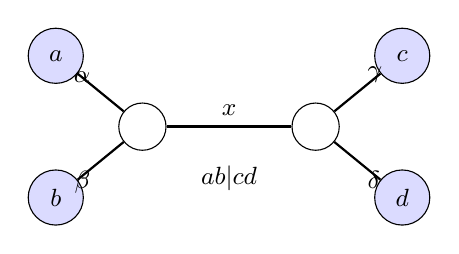
\begin{tikzpicture}[
  every node/.style={font=\small},
  leaf/.style={circle,draw,fill=blue!14,minimum size=7mm},
  hid/.style={circle,draw,fill=white,minimum size=6mm}
]
\node[hid] (u) at (0,0) {};
\node[hid] (v) at (2.2,0) {};
\node[leaf] (a) at (-1.1,0.9) {$a$};
\node[leaf] (b) at (-1.1,-0.9) {$b$};
\node[leaf] (c) at (3.3,0.9) {$c$};
\node[leaf] (d) at (3.3,-0.9) {$d$};
\draw[thick] (a)--node[above left] {$\alpha$} (u);
\draw[thick] (b)--node[below left] {$\beta$} (u);
\draw[very thick] (u)--node[above] {$x$} (v);
\draw[thick] (v)--node[above right] {$\gamma$} (c);
\draw[thick] (v)--node[below right] {$\delta$} (d);
\node at (1.1,-0.65) {$ab|cd$};
\end{tikzpicture}

  \caption{quartet 树 $ab|cd$：叶节点 $a,b$ 在内部边一侧，$c,d$ 在另一侧。}
  \label{fig:quartet}
\end{figure}

\begin{lemma}[树度量满足 four-point condition]
\label{lem:four_point_necessary}
任意加性树度量都满足 four-point condition。
\end{lemma}

\begin{proof}
任取四个叶节点 $a,b,c,d$。若它们在树上的最小连通子树没有内部边，即呈星形退化，则三项 $S_1,S_2,S_3$ 相等。否则该最小子树含一条内部边，诱导出一个 quartet 分裂。以\cref{fig:quartet}的 $ab|cd$ 为例，设内部边长度为 $x>0$，四条 pendant 边长度分别为 $\alpha,\beta,\gamma,\delta$。则
\begin{align}
  d_{ab}+d_{cd} &= (\alpha+\beta)+(\gamma+\delta),\\
  d_{ac}+d_{bd} &= (\alpha+x+\gamma)+(\beta+x+\delta)
                 = \alpha+\beta+\gamma+\delta+2x,\\
  d_{ad}+d_{bc} &= (\alpha+x+\delta)+(\beta+x+\gamma)
                 = \alpha+\beta+\gamma+\delta+2x.
\end{align}
因此后两项相等且大于第一项。其他分裂情形只是重命名节点，结论相同。
\end{proof}

\begin{proposition}[quartet 分裂的判别]
\label{prop:quartet_split}
若四点树度量中
\begin{equation}
  d_{ab}+d_{cd} < d_{ac}+d_{bd}=d_{ad}+d_{bc},
\end{equation}
则四点的非退化分裂为 $ab|cd$，内部边长度为
\begin{equation}
  x=\frac{1}{2}\left(d_{ac}+d_{bd}-d_{ab}-d_{cd}\right).
\end{equation}
\end{proposition}

\begin{proof}
由\cref{lem:four_point_necessary}证明中的 quartet 表达式，较小的和对应同侧叶对，较大两项比它多出 $2x$，故内部边长度如上。
\end{proof}

\section{与隐藏树重构的关系}

Four-point condition 的意义在于：即使内部节点不可观测，叶节点间距离仍然包含“哪些叶子共享近端分支”的信息。例如 $ab|cd$ 表示 $a,b$ 的路径在进入内部边前先汇合，$c,d$ 也先汇合。通过多个 quartet 的一致性，可以拼接出整棵隐藏树。

这解释了 leaf-only 场景不能只用 MST 的原因。MST 在叶节点集合上输出的是一棵叶节点树；hidden tree reconstruction 则允许新建内部节点，使输出树的叶间距离匹配输入距离。二者优化对象不同：
\begin{align}
  \text{MST:}\quad &\min_{T\text{ spans }L}\sum_{e\in T}\widehat d_e,\\
  \text{hidden tree:}\quad &\text{find }(\widetilde T,\widetilde w)\text{ such that }
  d_{\widetilde T}(i,j)\approx \widehat d_{ij},\ i,j\in L.
\end{align}

\section{四叶节点数值示例}

\begin{example}[判断 quartet]
设叶节点距离为
\[
\begin{array}{c|cccc}
 & a&b&c&d\\ \hline
a&0&2&5&5\\
b&2&0&5&5\\
c&5&5&0&2\\
d&5&5&2&0
\end{array}
\]
计算
\[
S_1=d_{ab}+d_{cd}=4,\quad
S_2=d_{ac}+d_{bd}=10,\quad
S_3=d_{ad}+d_{bc}=10.
\]
最大值出现两次，且 $S_1$ 最小，因此分裂为 $ab|cd$。内部边长度为 $(10-4)/2=3$。若四条 pendant 边均为 $1$，内部边为 $3$，正好得到该距离矩阵。
\end{example}

\begin{exercise}[给定矩阵判断 four-point condition]
对距离矩阵
\[
\begin{array}{c|cccc}
 &1&2&3&4\\ \hline
1&0&4&7&7\\
2&4&0&7&7\\
3&7&7&0&2\\
4&7&7&2&0
\end{array}
\]
判断是否满足 four-point condition，并给出 quartet 分裂与内部边长度。
\end{exercise}

\section{本章小结}

加性树度量把树结构编码进两两距离。Four-point condition 是树度量的基本判据：对任意四点，三种配对距离和的最大值至少出现两次；非退化时，较小项揭示 quartet 分裂。该条件使我们能够从叶节点距离中推断隐藏内部结构，也解释了为什么仅在叶节点上求 MST 无法恢复隐藏分支点。

\section*{思考题}
\begin{enumerate}
  \item 证明：若四个叶节点构成星形树，则 $S_1=S_2=S_3$。
  \item 若观测距离含噪，$S_2$ 与 $S_3$ 不再完全相等，应如何设置容差判断 quartet？
  \item Four-point condition 是树度量的必要条件。查阅 Buneman 相关结果，思考它在有限度量上是否也是充分条件。
  \item 在配电网中，哪些物理因素可能使叶间阻抗距离偏离精确树度量？
\end{enumerate}
